\subsection{Special Matchings}

\begin{definition}
	A \emph{matching} on a graph is an involution $M:V\to V$ s.t. $(v,M(v))\in E$ for all $v$. Take $G$ to be the Hasse diagram of a poset $P$. A \emph{special matching} is a matching such that for all $x,y\in P$, $x\lessdot y\implies M(x)\leq M(y)$.
\end{definition}
\begin{remark}
	For graded poset $P$, if $x\lessdot y$ and $x\lessdot M(x)$, then $y\lessdot M(y),M(x)\lessdot M(y)$.
\end{remark}
\begin{example}
	
\end{example}
\begin{theorem}\label{thm:sm_exists}
	Let $(W,S)$ be a Coxeter system, $u\leq v\in W$ and $s\in D(v)\setminus D(u)$. Let $M(x)=sx$ for any $x\in [u,v]$. Then $M$ is a special matching.
\end{theorem}
\begin{proof}
	If $w<v$ and $s\in D(w)$, then $sw\leq v$. Therefore $M$ is a matching.

Now take $x\lessdot y\in [u,v]$, want to show that $sx\leq sy$.	

(1) If $s\in D(x)\cap D(y)$, then $y$ has reduced word expression $ss_1\cdots s_k$. We can take a subword to get $x$, which will be $x=s s_1\cdots\hat s_i\cdots s_k$. Therefore $sx=s_1\cdots\hat s_i\cdots s_k$ is a subword of $sy=s_1\cdots s_k$.

(2) If $s\notin D(x)\cup D(y)$.

(3) If $s\in D(x)\setminus D(y)$.

(4) If $s\in D(y)\setminus D(x)$, then $M(x)=y$.

	
\end{proof}
\begin{corollary}
	The interval $[1,v$ always have a special matching.
\end{corollary}
\begin{remark}
	Not all special matching can be obtained as in \Cref{thm:sm_exists}.
\end{remark}
\begin{theorem}
	Let $M$ be a special matching of $[1,v]$. For $u\leq v$, we have%
	\begin{equation}
		R_{u,v} = q^c R_{M(u),M(v)}+ (q^c-1) R_{u,M(v)}
	\end{equation}
	where $c=1$ if $M(u)\gtrdot u$.
 \end{theorem}
 \begin{example}
 \[R_{1,14}=qR_{3,11}+(q-1)R_{1,11}\]
 \[R_{1,11}=q\underbrace{R_{2,8}}_{0}+(q-1)R_{1,8}=(q-1)^3\]
 \[R_{3,11}=q \underbrace{R_{6,8}}_{0} + (q-1)R_{3,8}=(q-1)^2\]
 \[R_{1,14}=q(q-1)^2+(q-1)^4\]
 	\begin{center}
 		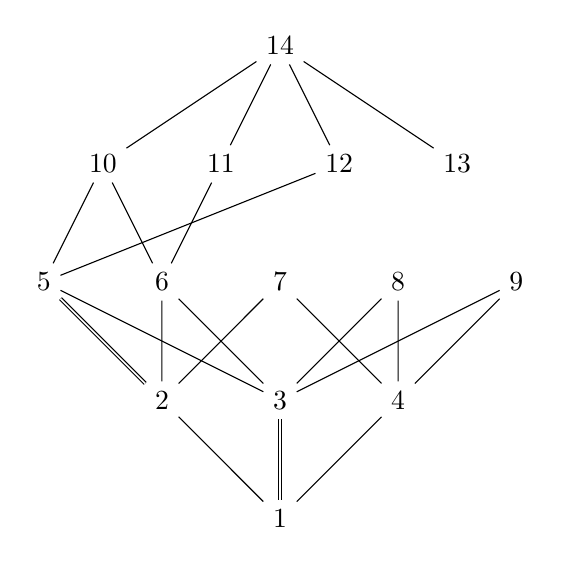
\begin{tikzpicture}[scale=1.5]
 			\node (1) at (0,0) {1};
 			\node (2) at (-1,1) {2};
 			\node (3) at (0,1) {3};
 			\node (4) at (1,1) {4};
 			\node (5) at (-2,2) {5};
 			\node (6) at (-1,2) {6};
 			\node (7) at (0,2) {7};
 			\node (8) at (1,2) {8};
 			\node (9) at (2,2) {9};
 			\node (10) at (-1.5,3) {10};
 			\node (11) at (-.5,3) {11};
 			\node (12) at (.5,3) {12};
 			\node (13) at (1.5,3) {13};
 			\node (14) at (0,4) {14};
 			
 			\draw (1)--(2);
 			\draw [double] (1)--(3);
 			\draw (1)--(4);
 			\draw [double](2)--(5);
 			\draw (2)--(6);
 			\draw (2)--(7);
 			\draw (3)--(5);
 			\draw (3)--(6);
 			\draw (3)--(8);
 			\draw (3)--(9);
 			\draw (4)--(7);
 			\draw (4)--(8);
 			\draw (4)--(9);
 			\draw (5)--(10);
 			\draw (5)--(12);
 			\draw (6)--(10);
 			\draw (6)--(11);
 			
 			
 			\draw (10)--(14);
 			\draw (11)--(14);
 			\draw (12)--(14);
 			\draw (13)--(14);
 		\end{tikzpicture}
 	\end{center}
 \end{example}